\section{Verwendete Verteilungen}
Zun�chst werden wir die Verteilungen vorstellen, die in dieser Arbeit verwendet werden, und die wichtigsten Eigenschaften vorstellen.
\\

\begin{defini}
Eine Zufallsvariable $X:\Omega\to \mathbb{R}$ hei�t \textbf{exponentialverteilt zum Parameter $\lambda$} (kurz: $X \sim exp(\lambda)$), wenn sie die folgende Dichtefunktion besitzt:
	\begin{eqnarray*}
		f_\lambda(x)=
		\begin{cases}
			\lambda e^{-\lambda x} & \text{f�r } x\geq 0 \\ 	
			0 & \text{f�r } x<0 \\ 
		\end{cases}
	\end{eqnarray*}
\end{defini}

\begin{figure}[H]
   \centering
      \subfloat[Dichtefunktion]{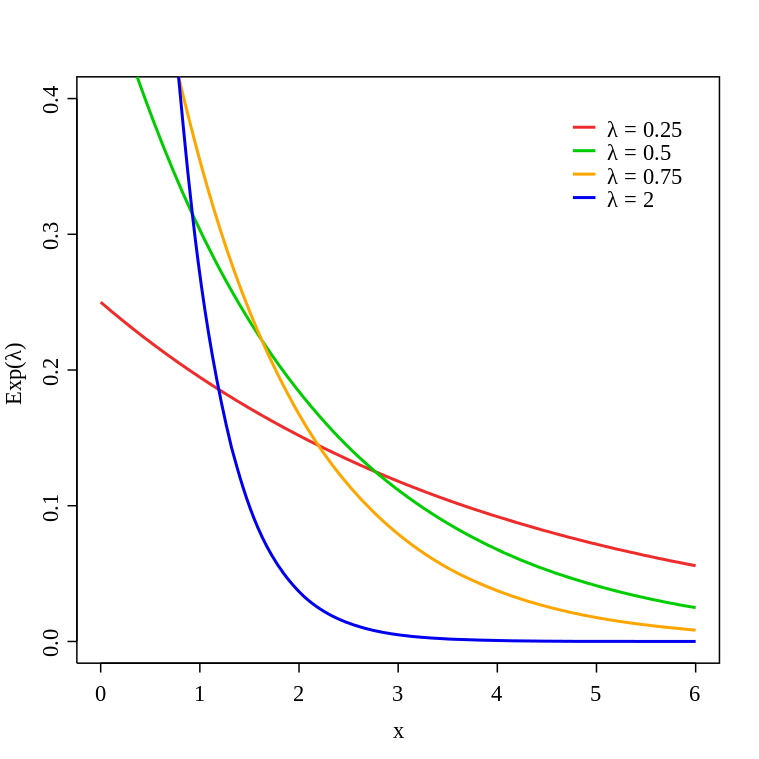
\includegraphics[width=0.39\textwidth]{./bilder/ExpDichteF}}\qquad
      \subfloat[Verteilungsfunktion]{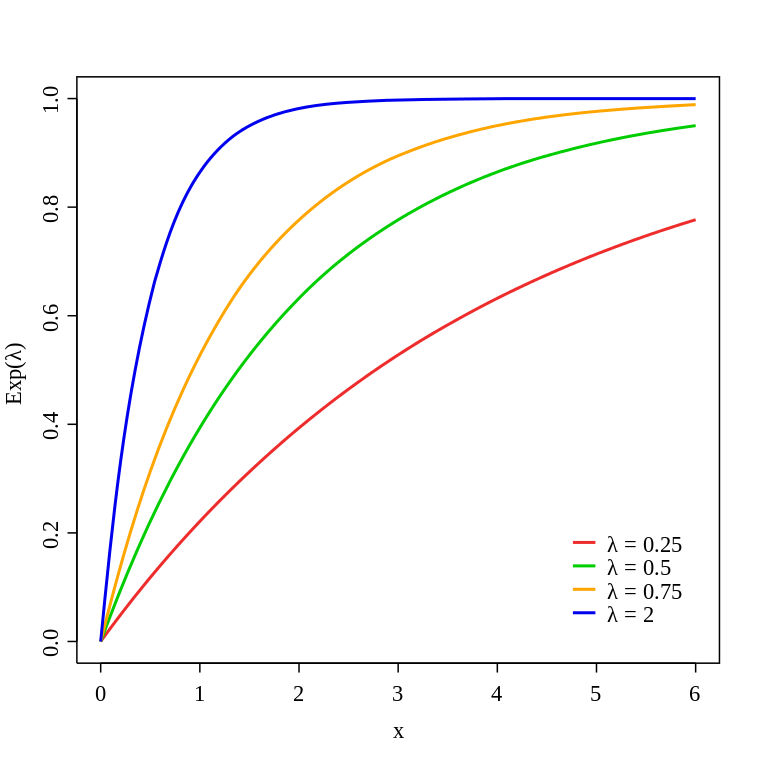
\includegraphics[width=0.39\textwidth]{./bilder/ExpVerteilungF}}
   \caption[Dichte- und Verteilungsfunktion der Exponentialverteilung]{Dichte- und Verteilungsfunktion der Exponentialverteilung}
\end{figure}

Sei $X \sim exp(\lambda)$ dann gilt:

\begin{enumerate}[label=(\roman{*})]
	\item Die Verteilungsfunktion von $X$ ist: 
	\begin{eqnarray*}
		F_X(x) = \int_{-\infty}^{x} f_{\lambda}(t) dt =
		\begin{cases}
			1-e^{-\lambda x} & \text{f�r } x\geq 0 \\ 	
			0 & \text{f�r } x<0 \\ 
		\end{cases}
	\end{eqnarray*}
	\item Der Erwartungswert ist:
	\begin{eqnarray*}
			\mathbb{E}(X) = \int_0^{\infty}\lambda xe^{-\lambda x} dx 
										= \left[-\frac{e^{-\lambda x}(\lambda x +1)}{\lambda}\right]^{\infty}_0
										= \frac{1}{\lambda}
	\end{eqnarray*}
	\item Die Varianz ist: 
	\begin{eqnarray*}
		Var(X) &=& \int_{0}^{\infty} \left(x-\frac{1}{\lambda}\right)^2 \lambda e^{-\lambda x} dx \\
					 &=& \int_{0}^{\infty} \left(x^2 -2x\frac{1}{\lambda} +  \frac{1}{\lambda ^2}\right) \lambda e^{-\lambda x} dx \\
					 &=& \lambda \int_{0}^{\infty} x^2e^{-\lambda x} dx- 2\int_{0}^{\infty}xe^{-\lambda x}dx +  \frac{1}{\lambda} \int_{0}^{\infty}e^{-\lambda x} dx \\
					 &=& \lambda \int_{0}^{\infty} x^2e^{-\lambda x} dx-\frac{2}{\lambda ^2} + \frac{1}{\lambda ^2} \\
					 &=& \lambda \big(\underbrace{\left[-\frac{1}{\lambda} x^2 e^{-\lambda x}\right]_0^{\infty}}_{\substack{0}} + \frac{2}{\lambda}\int_{0}^{\infty}xe^{-\lambda x}dx\big) - \frac{2}{\lambda ^2} \\
					 &=& \frac{2}{\lambda^2} - \frac{1}{\lambda^2} \\
					 &=& \frac{1}{\lambda^2}
	\end{eqnarray*}
	\item Die Exponentialverteilung ist ged�chtnislos (auch Nichtalterungseigenschaft genannt), d.h. f�r $X$ gilt:
	\begin{eqnarray*}
		\mathbb{P}(X> x+t\: | \: X > t) &=& \frac{\mathbb{P}(X> x+t, X > t)}{\mathbb{P}(X> t)} \\
					 &=& \frac{\mathbb{P}(X> x+t)}{\mathbb{P}(X> t)} \\
					 &=& \frac{e^{-\lambda (x+t)}}{e^{-\lambda t}} \\
					 &=& e^{-\lambda x} = \mathbb{P}(X> x)
	\end{eqnarray*}
\end{enumerate}

Die Exponentialverteilung hat die besondere Eigenschaft der Ged�chtnislosigkeit und es l�sst sich sogar zeigen, dass sie die einzige absolut stetige Verteilung\footnote{Im diskreten Fall ist dies die geometrische Verteilung.} mit dieser Eigenschaft ist:

\begin{lemmas} \label{expLemma} Sei X eine absolut stetige postive Zufallsvariable, dann gilt  $X \sim exp(\lambda)$ genau dann wenn f�r alle $x, t > 0$ gilt, dass
	\begin{eqnarray} \label{eq:ged}
		\mathbb{P}(X> x+t\: | \: X > t) = \mathbb{P}(X> x+t\: | \: X > t)
	\end{eqnarray}
\end{lemmas}

\textbf{Beweis:}
$\Rightarrow$ Sei $X \sim exp(\lambda)$ dann gilt:
	\begin{eqnarray*}
		\mathbb{P}(X> x+t\: | \: X > t) &=& \frac{\mathbb{P}(X> x+t, X > t)}{\mathbb{P}(X> t)} \\
					 &=& \frac{\mathbb{P}(X> x+t)}{\mathbb{P}(X> t)} \\
					 &=& \frac{e^{-\lambda (x+t)}}{e^{-\lambda t}} \\
					 &=& e^{-\lambda x} = \mathbb{P}(X> x)
	\end{eqnarray*}

$\Leftarrow$ Sei umgekehrt X eine absolut stetige Zufallsvariable, die die Gleichung \ref{eq:ged} erf�llt. Wir definieren $g(x) := \mathbb{P}(X > x)$. F�r $x, y > 0$ gilt:

\begin{eqnarray*}
	g(x + t) &=& \mathbb{P}(X > x + y) \\
					 &=& \mathbb{P}(X > x + y \: | \: X > y) \mathbb{P}(X > y) \\
					 &=& \mathbb{P}(X > x) \mathbb{P}(X > y) = g(x)g(y)
\end{eqnarray*}
Durch n-fache Anwendung folgt f�r alle $n \in \mathbb{N}$:

\begin{eqnarray*}
g(1) = g\big( \underbrace{\frac{1}{n} + ... + \frac{1}{n}}_{\substack{n-mal}} \big) = \left(g\big(\frac{1}{n}\big)\right)^n
\end{eqnarray*}
und somit insbesondere auch $g(\frac{1}{n}) = (g(1))^\frac{1}{n}$. Da X nur positive Werte annimmt, existiert ein $n \in \mathbb{N}$ mit $g(1/n) > 0$. Au�erdem existiert wegen $0 < g(1) \leq 1$, ein $\lambda \geq 0$ mit $g(1) = e^{-\lambda}$. F�r beliebige $p, q \in \mathbb{N}$ gilt 
\begin{eqnarray*}
	g(\frac{p}{q}) = g(\frac{1}{q})^p = g(1)^{\frac{p}{q}}
\end{eqnarray*}
und somit $g(r) = e^{-\lambda r}$ f�r alle $r \in \mathbb{Q}^+$. Aufgrund der Stetigkeit folgt daraus
\begin{eqnarray*}
	g(x) = e^{-\lambda x}
\end{eqnarray*}
\qed

\begin{defini}
Eine diskrete Zufallsvariable $X:\Omega\to \mathbb{N}$ hei�t \textbf{poissonverteilt zum Parameter $\lambda \in \mathbb{R}_{>0}$} (kurz $X\sim Poi(\lambda)$), wenn gilt:

\begin{eqnarray*}
	P_{\lambda}(k) := \mathbb{P}(X=k) = \frac{\lambda^k}{k!}e^{-\lambda}, k=0,1,2,...
\end{eqnarray*}
\end{defini}

Die Poisson-Verteilung hat folgende Eigenschaften:

\begin{enumerate}[label=(\roman{*})]
	\item Die Verteilungsfunktion der Poisson-Verteilung ist: 
	\begin{eqnarray*}
		F_{\lambda}(n) = \sum_{k=0}^{n} P_{\lambda}(k) = e^{-\lambda} \sum_{k=0}^{n} \frac{\lambda^k}{k!}
	\end{eqnarray*}
	\item Der Erwartungswert ist:
	\begin{eqnarray*}
			\mathbb{E}(X) &=& \sum_{k=0}^{\infty} k\frac{\lambda^k}{k!} e^{-\lambda}  
										=  0 + \sum_{k=1}^{\infty} k\frac{\lambda^k}{k!} e^{-\lambda} \\
										&=& \lambda e^{-\lambda} \sum_{k=1}^{\infty} \frac{\lambda^{k-1}}{(k-1)!} \\
										&=& \lambda e^{-\lambda} \sum_{i=0}^{\infty} \frac{\lambda^i}{i!} 
										= \lambda e^{-\lambda} e^{\lambda} 
										= \lambda
	\end{eqnarray*}
	
	Der Parameter $\lambda$ der Poisson-Verteilung kann also, als die erwartete Ereignish�ufigkeit pro Zeiteinheit interpretiert werden.
	
	\item Die Varianz ist: 
	\begin{eqnarray*}
		\mathbb{E}(X^2) &=& \sum_{k=0}^{\infty} k^2 \frac{\lambda^k}{k!} e^{-\lambda} \\
										&=& e^{-\lambda} \sum_{k=1}^{\infty} k \frac{\lambda^{k}}{(k-1)!} \\
										&=& e^{-\lambda} \sum_{k=1}^{\infty} \frac{((k-1)+1)\lambda^{k}}{(k-1)!} \\
										&=& e^{-\lambda} \sum_{k=2}^{\infty} \frac{\lambda^{k}}{(k-2)!} + e^{-\lambda} \sum_{k=1}^{\infty} \frac{\lambda^{k}}{(k-1)!} \\
										&=& \lambda^2 e^{-\lambda} \sum_{k=2}^{\infty} \frac{\lambda^{k-2}}{(k-2)!} + \lambda e^{-\lambda} \sum_{1}^{\infty} \frac{\lambda^{k-1}}{(k-1)!} \\
										&=& \lambda^2+\lambda \\ \\
						 Var(X) &=& \mathbb{E}(X^2) - \mathbb{E}(X)^2 = \lambda^2+\lambda - \lambda^2 = \lambda
	\end{eqnarray*}
	\item Seien $X_1$ und $X_2$ unabh�ngige poissonverteilte Zufallsvariablen mit $X_1\sim Poi(\lambda _1)$ und $X_2\sim Poi(\lambda _2)$, dann gilt f�r $X := X_1 + X_2 $:
		\begin{eqnarray*}
			\mathbb{P}(X=x) &=& \sum_{k=0}^{x} \mathbb{P}(X_1=k)\mathbb{P}(X_2=x-k) \\
											&=& e^{-\lambda_1}e^{-\lambda_2} \sum_{k=0}^{x} \frac{\lambda _{1} ^k}{k!} \frac{\lambda _{2} ^{x-k}}{(x-k)!} \\
											&=& \frac{e^{-(\lambda_1+\lambda_2)}}{x!} \sum_{k=0}^{x} \frac{x!}{k!(x-k)!}\lambda _{1}^k \lambda _{2}^{x-k} \\
											&=& e^{-(\lambda_1+\lambda_2)} \frac{(\lambda _{1} + \lambda _{2})^x}{x!} \\
				\Rightarrow  X &\sim & Poi(\lambda _1 + \lambda _2) 
		\end{eqnarray*}
		Das hei�t die Summe von poissonverteilten Zufallsvariablen ist wieder poissonverteilt.
	\end{enumerate}

Die Poisson-Verteilung hat au�erdem eine besondere Bedeutung, da sie unter den richtigen Voraussetzungen die Grenzverteilung der Binomialverteilung ist. Dieser Zusammenhang wird in folgendem Lemma verdeutlicht: \\

\begin{lemmas} Sei $X \sim B_{n,p}(k)$ eine binomialverteilte Zufallsgr��e. Wenn f�r $n \rightarrow \infty$ und $p \rightarrow 0$ gilt, dass der Erwartungswert $np$ gegen eine von $n$ unabh�ngige Konstante $\lambda$ konvergiert, dann konvergiert die Verteilungsfunktion von X gegen die Verteilungsfunktion einer, zum Parameter $\lambda$, poissonverteilten Zufallsgr��e.
\end{lemmas}

\textbf{Beweis:}
Wir zeigen, dass der Grenzwert $n\rightarrow \infty$ der Verteilungsfunktion einer binomialverteilten Zufallsvariable an der Stelle k, gegen den Wert einer poissonverteilten Zufallsvariablen an der Stelle k geht.

	\begin{eqnarray*}
		\lim_{\substack{n\rightarrow \infty\\p\rightarrow 0}} \mathbb{P}(X=k) &=& \lim_{\substack{n\rightarrow \infty\\p\rightarrow 0}}\binom{n}{k} p^k(1-p)^{n-k}\\
		&=& \lim_{\substack{n\rightarrow \infty\\p\rightarrow 0}} \frac{n!}{k!(n-k)!} \left(\frac{\lambda}{n}\right)^k \left(1-\frac{\lambda}{n}\right)^{n-k} \\
		&=& \frac{\lambda ^k}{k!} \lim_{\substack{n\rightarrow \infty\\p\rightarrow 0}} \underbrace{\left(\frac{n(n-1)(n-2)...(n-k+1)}{n^k}\right)}_{\rightarrow 1} \underbrace{\left( 1-\frac{\lambda}{n}\right)^{n}}_{\rightarrow e^{-\lambda}} \underbrace{\left(1-\frac{\lambda}{n}\right)^{-k}}_{\rightarrow 1} \\
		&=& \frac{\lambda ^k e^{-\lambda}}{k!}		
	\end{eqnarray*}
\qed